\section{Software Design and Implementation}

This design outlines the software developed for a Raspberry Pi, consisting of two main components: a C++ backend responsible for managing LoRa communication, and a Flutter frontend that delivers a user-friendly interface for message handling and display.

\begin{figure}[H]
\centering
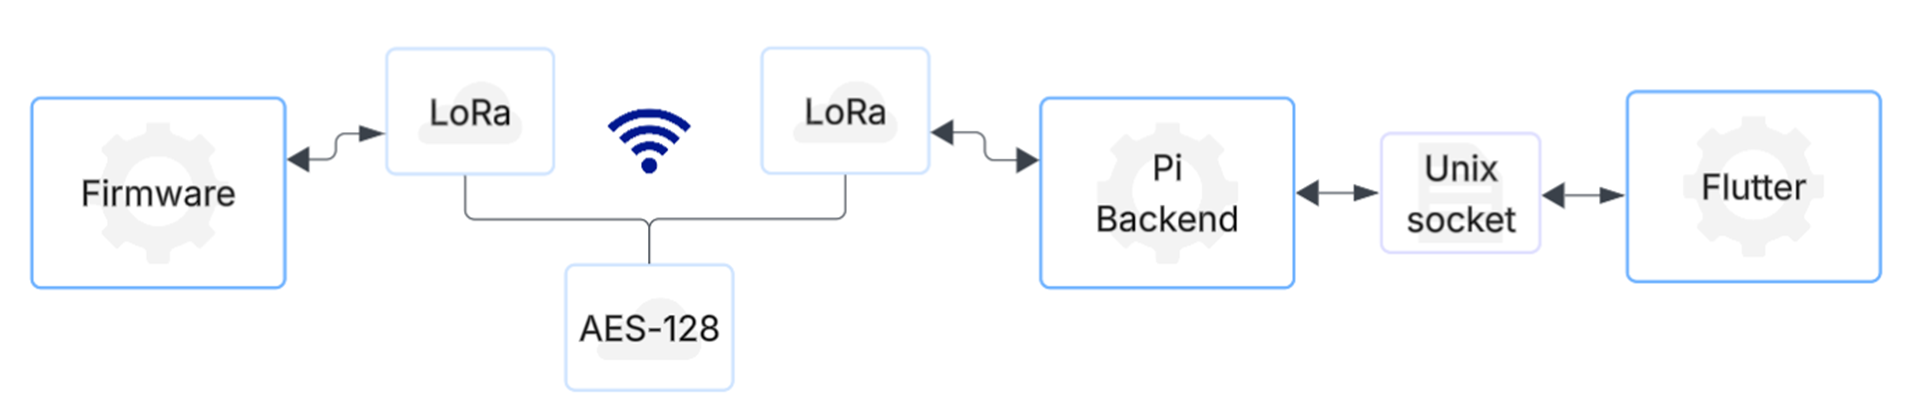
\includegraphics[width=0.45\textwidth]{images/lora-shield.png}
\caption{Overview of the software design}\label{fig:lora-shield}
\end{figure}

\subsection{Backend Implementation}

The backend is implemented in C++ and is responsible for managing the core functionality of the LoRa communication system with the firmware. 
This script is currently designed to run on a Raspberry Pi (RPI), where a shield called the LoRa-GPS HAT~\cite{LoRa-GPS-HAT} is mounted. 
This shield includes a GPS module (not utilized in this project) and an RFM96 LoRa chip~\cite{LoRa module}, a low-power, 
long-range transceiver that operates in the 868\,MHz frequency band.

\subsection{LoRa Communication Layer}

The LoRa communication layer ensures that the backend can send and receive messages over the LoRa network.
Before communication can be established, the interface with the LoRa chip on the shield must be properly configured.

\textbf{SPI Initialization:}

\begin{enumerate}
  \item SPI must be enabled on the Raspberry Pi using the \texttt{raspi-config} utility.
  \item Once enabled, SPI is initialized in the code. The WiringPi library~\cite{WiringPi} is used to access the GPIO pins—specifically, 
  Pin~7 is configured as the interrupt (IRQ) pin for the LoRa chip. After the hardware connection is established, register-level communication is handled through implemented methods such as \texttt{read\_register} and \texttt{write\_register}. Additionally, the \texttt{write\_fifo} method is used to transfer data into the FIFO buffer of the LoRa transceiver.
\end{enumerate}

\textbf{Message Handling:} \\
To support message exchange with the firmware, 
we adapted the same communication library used by the firmware and tailored it to fit the backend's architecture. 
A consistent packet structure is required for interoperability. Each packet includes the following fields: 
\texttt{type}, \texttt{message\_id}, \texttt{fragment\_id}, \texttt{total\_fragments}, \texttt{length}, \texttt{data}, and \texttt{checksum}. 
This structure ensures reliable fragmentation, transmission, and validation of messages between the backend and firmware.
Then to make this more secure we used AES-128 encryption ~\cite{tiny-AES} in CTR mode to encrypt the data field of the packet. 

\subsection{Communication between the Backend and the Frontend}

To establish a smooth and efficient flow of communication between the backend and the frontend, a non-blocking Unix domain socket is used.
This approach enables asynchronous communication, allowing the system to perform multiple operations concurrently without blocking the main 
thread—an essential feature for real-time LoRa communication.

A corresponding socket is also implemented in the Flutter application, enabling the frontend to interact with the backend seamlessly 
and without interrupting its main execution thread.

\textbf{Receiving LoRa Packets from the Firmware:} \\
When a LoRa packet is received from the firmware, the backend handles it using the following sequence:

\begin{enumerate}
  \item An interrupt is immediately triggered by the LoRa module.
  \item The backend processes the received packet.
  \item The processed packet is forwarded to the frontend through the non-blocking Unix domain socket.
  \item The system remains responsive and ready to handle the next incoming LoRa packet.
\end{enumerate}

\subsection{Frontend implementation}

Below is an image showcasing the user interface. The frontend is implemented using Flutter~\cite{flutter}, which enables the development of a responsive and user-friendly UI.

\begin{figure}[H]
\centering
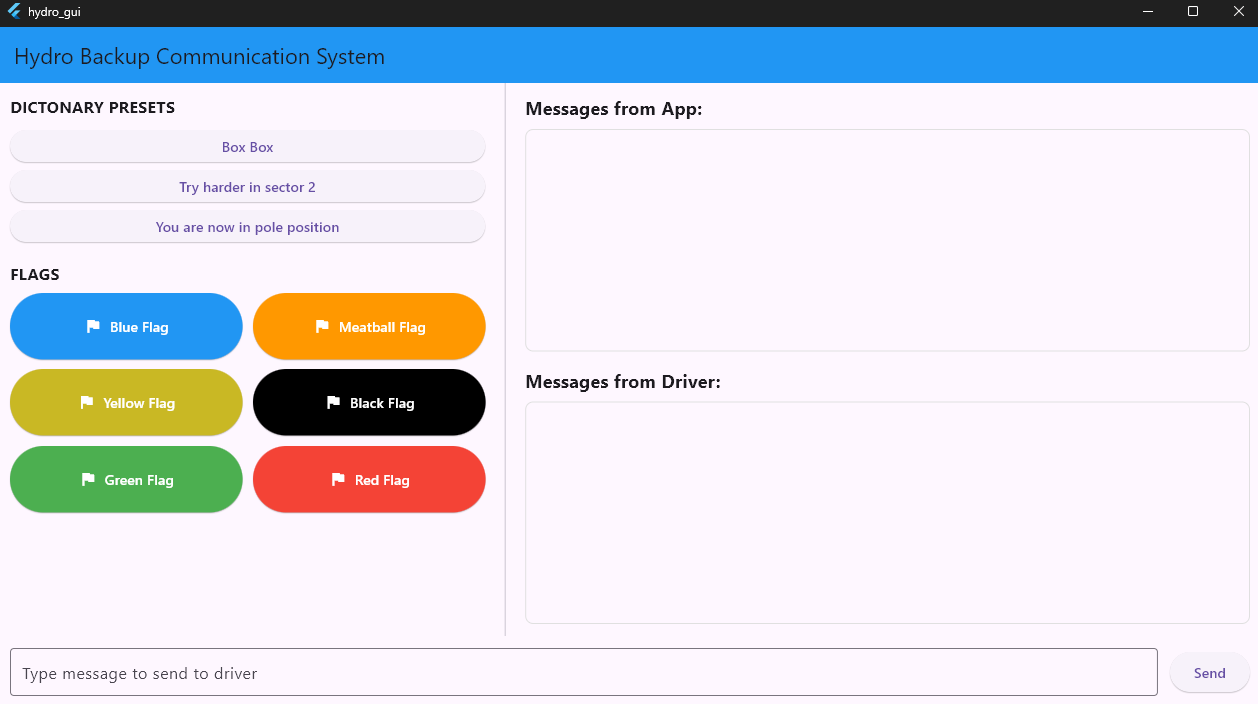
\includegraphics[width=0.45\textwidth]{images/frontend-design.png}
\caption{User interface}\label{fig:frontend-design}
\end{figure}

The interface is composed of several key elements:

\begin{itemize}
    \item Split-view layout with preset messages and flags on the left
    \item Dual message displays showing both sent/app and received messages
    \item An input field for composing custom messages
\end{itemize}

The preset messages and flags are designed for quick access, allowing the user to send predefined commands to the driver efficiently. 
Each flag is associated with a specific ID (e.g., the blue flag corresponds to \texttt{FLAG:1}). 
When the user taps a flag, the corresponding ID is sent to the backend, which forwards it to the firmware. 
The firmware then plays the appropriate \texttt{.wav} file stored on the Nucleo board.

For custom messages, the entered text is transmitted as raw data. 
The firmware receives this message and uses speech synthesis to convert the text into audio output.

On the right side of the interface, received messages from the backend are displayed. 
These may include system notifications, such as error reports or status pings to verify that the driver can receive and acknowledge incoming messages.
